\documentclass[12pt]{article}
\usepackage{graphicx} % Required for inserting images
\usepackage{hyperref}
\usepackage{makecell}
\usepackage{makeidx}
\usepackage{eurosym}
\usepackage{fancyhdr}
\usepackage{titlesec}
\usepackage{longtable}
\newcommand{\firstPage}{
    \thispagestyle{empty}
    \begin{figure}
    \centering
    
\includegraphics[scale=0.7]{Swellfish_logo.png}
    \end{figure}
    \author{
        \date{}
        \href{mailto://swellfish14@gmail.com}{swellfish14@gmail.com} \\
    } 
} 
\usepackage{hyperref}
\usepackage{array}
\usepackage{tabularx}
\usepackage{adjustbox}

\newcounter{verscount}
\setcounter{verscount}{0}
\newcommand{\addversione}[5]{
	\ifdefined\setversione
		\setversione{#1}
	\else\fi
	\stepcounter{verscount}
	\expandafter\newcommand%
		\csname ver\theverscount \endcsname{#1&#2&#3&#4&#5}
}

\newcommand{\listversioni}{
	\ifnum\value{verscount}>1
		\csname ver\theverscount \endcsname
		\addtocounter{verscount}{-1}
		\\\hline
		\listversioni
	\else
		\csname ver\theverscount \endcsname\\\hline
	\fi
}

\newcommand{\makeversioni}{
	\begin{center}
		\begin{tabularx}{\textwidth}{|c|c|X|X|X|}
		\hline
		\textbf{Versione} & \textbf{Data} & \textbf{Redattore} & \textbf{Verificatore} & \textbf{Descrizione} \\
		\hline
		\listversioni
		\end{tabularx}
	\end{center}
	\clearpage
}

\fancypagestyle{genericDocstyle}{
	\pagestyle{fancy}
	\lhead{
\includegraphics[width=1cm]{Swellfish_logo.png}}
	\rhead{Norme di progetto}
}

%\hypersetup{colorlinks=true,urlcolor=blue}

%\newcommand{\tableContent}{

	%{
		%\hypersetup{linkcolor=black}
		%\tableofcontents
	%}
%}
\graphicspath{ {../templates/img/} }

\begin{document}
\setcounter{tocdepth}{4}
\setcounter{secnumdepth}{4}
\title{Specifica Tecnica}

\firstPage
\pagebreak

\maketitle

\begin{center}
    \begin{tabular}{r | l}
		\multicolumn{2}{c}{\textit{Informazioni}}\\
		\hline
		
			\textit{Redattori} &
			[Davide Porporati, Elena Marchioro, Francesco Naletto]\makecell{}\\

			\textit{Revisori} &
			[Jude Vensil Braceros]\makecell{}\\
			\textit{Responsabili} &
			[Andrea Veronese]\makecell{}\\
		      \textit{Uso} & 
                [Esterno]\makecell{}\\
    \end{tabular}
\end{center}

\begin{center}
    \textbf{Descrizione}\\
	File contenente la specifica tecnica necessaria per la realizzazione del progetto. 
\end{center}

\pagebreak
\addversione{0.0.0}{09/08/2023}{Elena Marchioro}{Davide Porporati}{Creata struttura di base del documento}
\addversione{0.0.1}{01/09/2023}{Davide Porporati, Elena Marchioro}{Francesco Naletto}{Modificata tabella requisiti e informazioni principali}
\addversione{0.0.2}{04/09/2023}{Davide Porporati, Elena Marchioro}{Francesco Naletto}{Aggiornati i design pattern e caricato diagramma delle classi}
\addversione{0.0.3}{09/09/2023}{Davide Porporati, Elena Marchioro}{Claudio Giaretta}{Aggiornati i design pattern e revisionato il documento}
\addversione{1.0.0}{09/09/2023}{Davide Porporati, Elena Marchioro}{Francesco Naletto}{Aggiornati i diagrammi delle classi}
\addversione{1.0.1}{18/09/2023}{Davide Porporati, Elena Marchioro}{Francesco Naletto}{Aggiornati i diagrammi delle classi e aggiunte sezioni mancanti}
\addversione{1.0.2}{25/09/2023}{Davide Porporati, Elena Marchioro}{Francesco Naletto}{Aggiornati i diagrammi UML dopo revisione PB}
\makeversioni

\tableofcontents

\pagebreak

\graphicspath{ {./UML/images/} }

\section{Introduzione}

\subsection{Scopo del documento}
Nel seguente documento vengono illustrate e motivate le scelte architetturali decise. Vengono riportati i diagrammi delle classi per l'architettura e le funzionalità principali,
il diagramma ER della base di dati e infine una sezione dalla quale si può verificare lo stato di avanzamento del prodotto grazie a una tabella che illustra
i requisiti soddisfatti.

\subsection{Scopo del prodotto}
L’obiettivo di SWEllfish e dell’azienda ImolaInformatica S.p.A. è lo sviluppo di un sistema per l’ottimizzazione dell’illuminazione, attraverso la realizzazione di una WebApp che permetta a degli utenti registrati di gestire l'impianto di illuminazione
di un'area in modo manuale e automatico. Nel documento viene riportata l'architettura del sistema per i vari servizi e i design pattern utilizzati.

\subsection{Riferimenti}
\subsubsection{Riferimenti normativi}
\begin{itemize}
	\item Norme di progetto
	\item Capitolato d'appalto C2 - \href{https://www.math.unipd.it/~tullio/IS-1/2022/Progetto/C2.pdf}{Lumos Minima}
\end{itemize}
\subsubsection{Riferimenti informativi}
\begin{itemize}
	\item Analisi dei requisiti
	\item Slide P2 del corso di ingegneria del software - \href{https://www.math.unipd.it/~rcardin/swea/2023/Diagrammi%20delle%20Classi.pdf}{Diagrammi delle classi}
	\item Slide P4 del corso di ingegneria del software - \href{https://www.math.unipd.it/~rcardin/sweb/2022/L02.pdf}{Progettazione: il pattern Model-View-Controller e derivati}
\end{itemize}
\section{Tecnologie Utilizzate}
\subsection{Front-end}
Per realizzare il frontend, ovvero la GUI del sistema, le seguenti tecnologie sono state impiegate:
\begin{itemize}
	\item React: libreria JavaScript per creare GUI
	\item Typescript: linguaggio basato su JavaScript, offre migliore scalabilità rispetto a JS
	\item Bulma: framework CSS, reponsible e modulare, basato su Flexbox.
\end{itemize}

\subsection{Back-end}
\begin{itemize}
	\item Node.JS: runtime di tipo JavaScript
	\item Express: framework per Node.JS
	\item Axios: client HTTP per Node.JS di tipo "promise-based"
	\item Sequelize: ORM tool per MariaDB, utilizzato per modellare i dati ed effettuare associazioni
	\item Cron: modulo di node, funge da scheduler e viene impiegato per creare task ad esecuzione automatica
\end{itemize}

\subsection{Database}
Il database implementato è di tipo relazionale, ed è stato implementato utilizzando MariaDB e HeidiSQL.
\subsection{Interfacciamento Lampioni/Sensori}
Per realizzare l'interfacciamento con i sensori e i lampioni a sistema le seguenti tecnologie sono state impiegate:
\begin{itemize}
	\item Python
	\item API-rest 
\end{itemize}

\section{Architettura del prodotto}

\subsection{Diagramma delle classi}
\subsection{Back-End}
\includegraphics[width=475pt]{Back-End.png}
\subsubsection{Model}
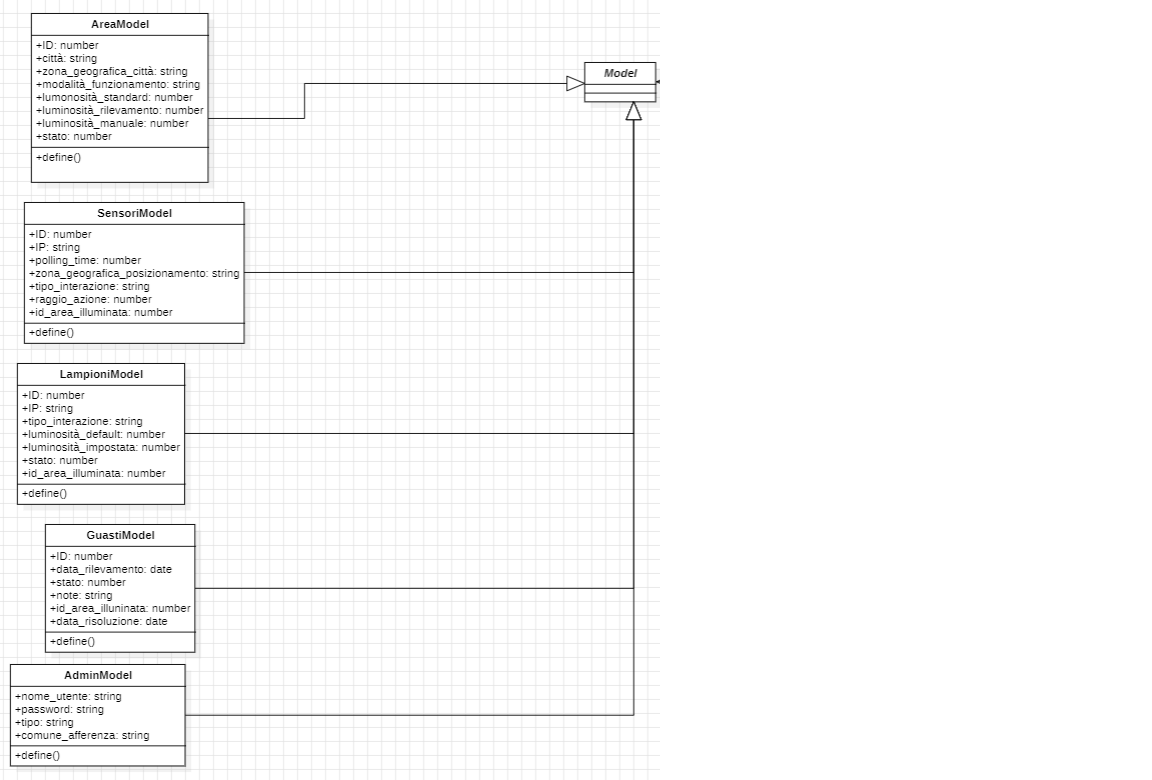
\includegraphics[width=475pt]{Model.png}
\subsubsection{Router}
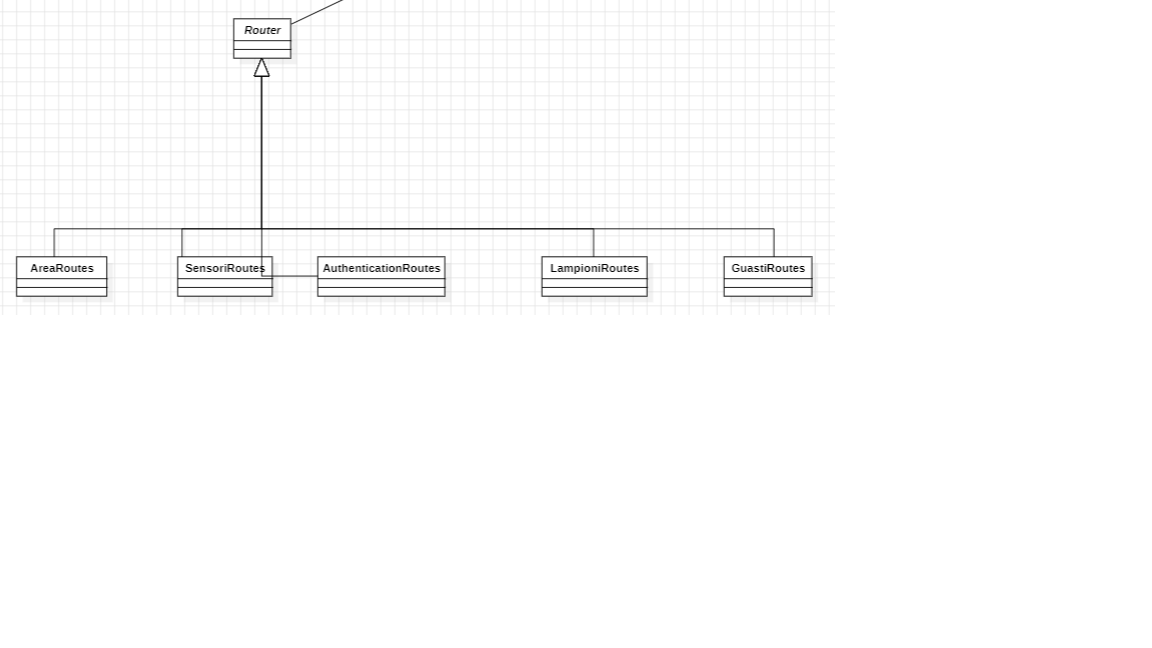
\includegraphics[width=475pt]{Router.png}
\subsubsection{Controller}
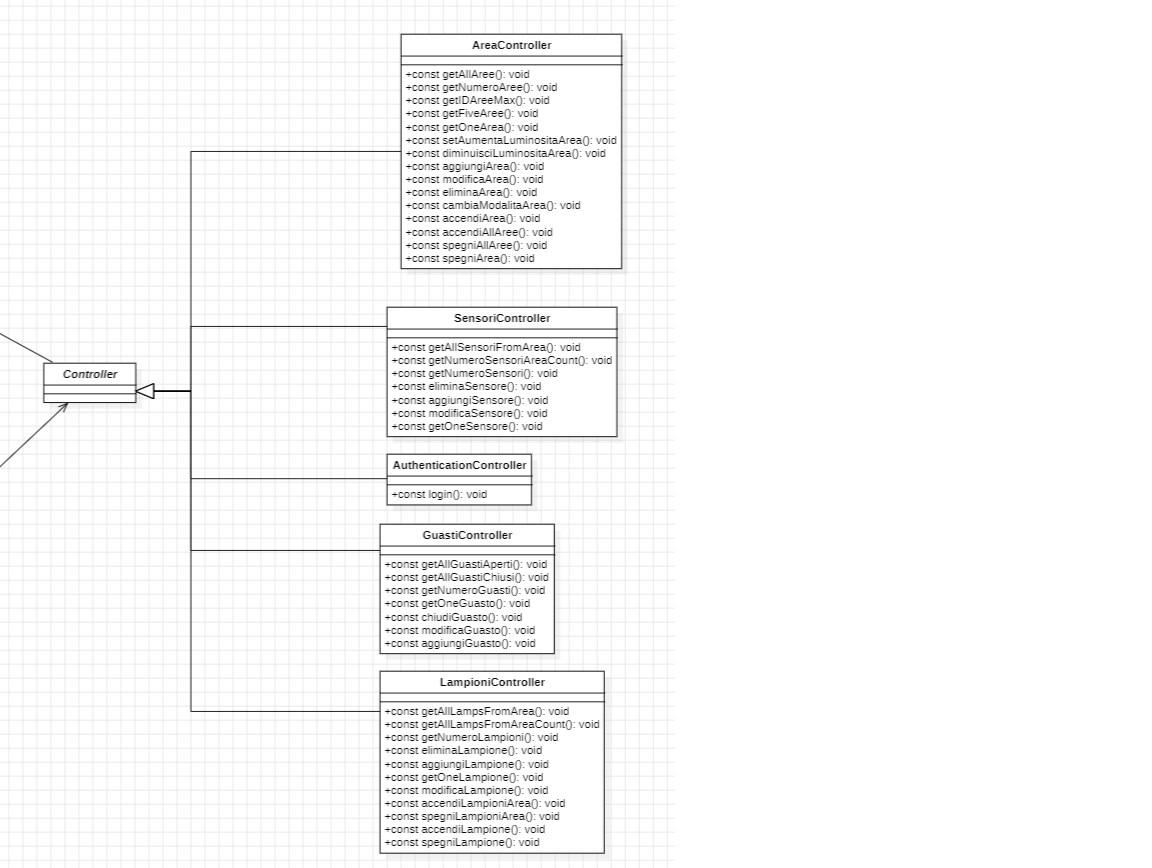
\includegraphics[width=475pt]{Controller.png}
\subsubsection{Service}
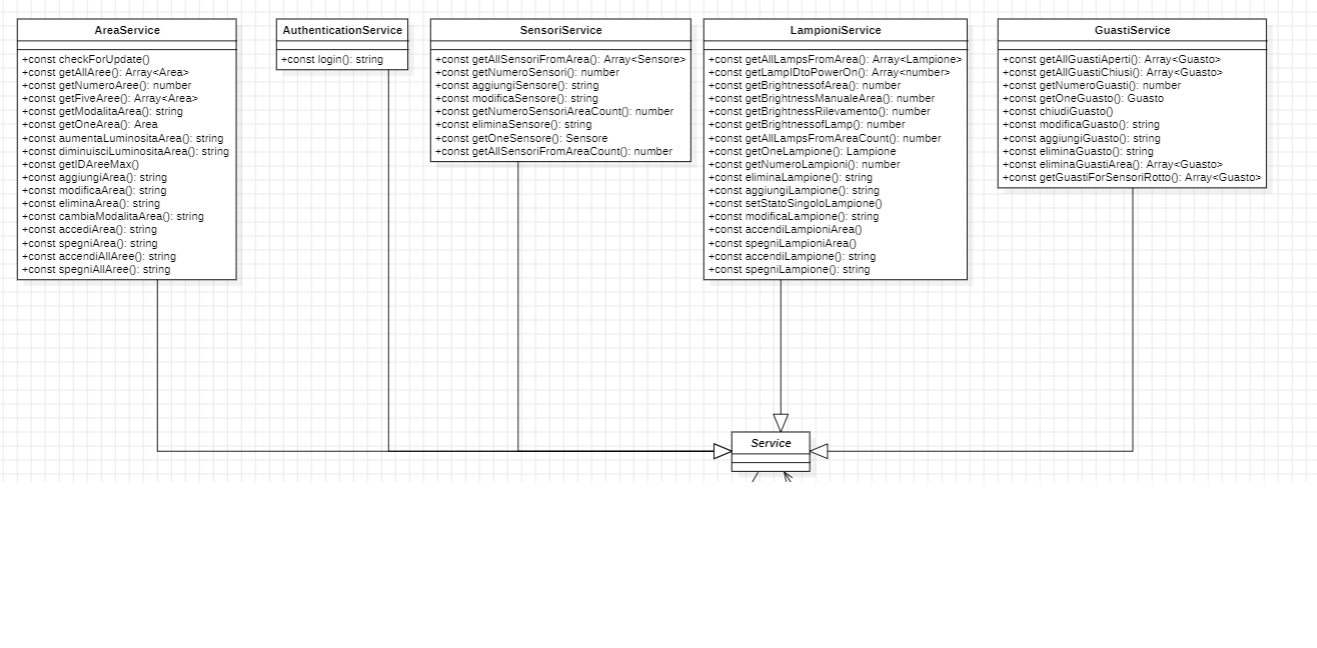
\includegraphics[width=475pt]{Service.png}
\clearpage
\subsection{Front-End}
\includegraphics[width=475pt]{Front-End.png}
\clearpage
\includegraphics[width=475pt]{Front-End2.png}
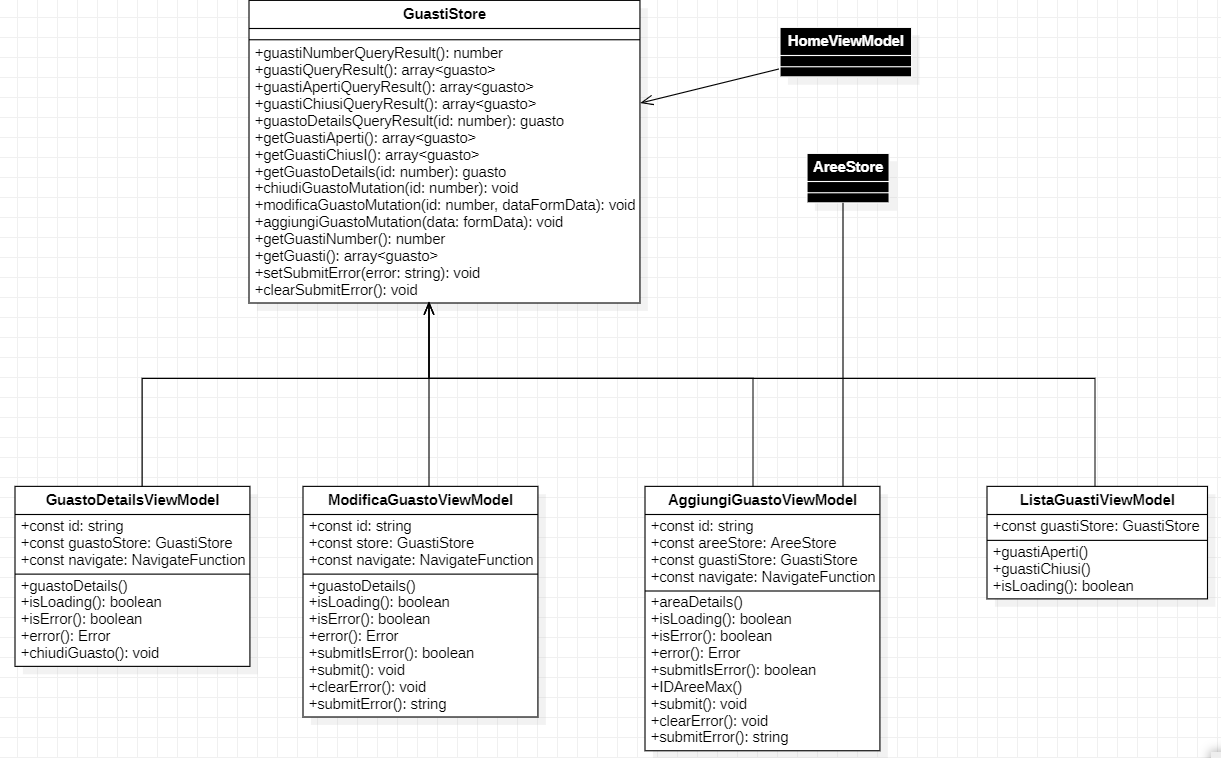
\includegraphics[width=475pt]{Guasti.png}


\subsection{Design Pattern}
\subsubsection{Back-end}
Per il backend è stato utilizzato il seguente pattern:
	\begin{itemize}
		\item Router Controller Service Pattern:
			Il design pattern dell'API Router-Controller-Service è un modello di architettura del software comunemente utilizzato nelle applicazioni web per strutturare e organizzare il codice responsabile della gestione delle richieste e delle risposte HTTP. Questo pattern aiuta a mantenere la separazione delle responsabilità e migliora la modularità e la manutenibilità dell'applicazione.

			Il pattern è composto dai seguenti componenti:
			\begin{itemize}
				\item Router: componente che si occupa di effettuare il routing verso il controller adatto
				\item Controller: componente che elabora la rischiesta ricevuta dal Router. Si appoggia alla classe Service per eseguire le operazioni.
				\item Service: componente che esegue la logica dell'applicazione.
			\end{itemize}
			Ecco come funziona il pattern in pratica:
			\begin{itemize}
				\item Un client invia una richiesta HTTP alla tua applicazione;
				\item Il componente Router riceve la richiesta e determina quale Controller deve gestirla in base all'URL e al metodo HTTP;
				\item Il Controller selezionato elabora la richiesta. Se necessario, chiama i metodi del livello di Servizio per eseguire la logica aziendale e le operazioni sui dati.
				\item Il Controller costruisce una risposta HTTP, che viene inviata al client.
			\end{itemize}		
	\end{itemize}
\subsubsection{Front-end}
Per il frontend si sono utilizzati i pattern:
\begin{itemize}
	\item Observer Pattern:
	\begin{itemize}
		\item Scopo: definire una dipendenza fra oggetti, riflettendo la modifica di un oggetto sui dipendenti.
		\item Motivazione: mantenere la consistenza fra oggetti e definire come implementare la relazione di dipendenza.
	\end{itemize}
	\item Dependency Injection: le dipendenze sono tracciate e passate agli oggetti tramite costruttore.
	 Questo pattern è stato impiegato perchè facilita il tracciamento delle dipendenze e agevola la fase di testing, rendendo più semplice il mocking.
	\item Model View ViewModel (MVVM): è un modello di architettura del software che facilita la separazione dello sviluppo dell'interfaccia grafica, ovvero la GUI,
sia tramite un linguaggio di markup o un codice GUI, dallo sviluppo del business logic o logica back-end in modo tale che la vista non dipenda da alcuna piattaforma di modello specifica.
I componenti del modello MVVM:	
	\begin{itemize}
		\item Model: nel nostro cosa è rappresentato nel file "api-types.ts"
		\item View: viene definita tramite un template HTML accessibile nella cartella "Public". Per ogni view la parte root del template viene sostituita con la vista corrispondente
		\item ViewModel: viene rappresentato dalle classi TypeScript utilizzate per gestire gli eventi della vista e aggiornare il modello di conseguenza. Ne è un esempio la classe "AreeViewModel", che gestisce la visualizzazione della lista delle aree presenti a sistema.
	\end{itemize}
Il pattern implementato dal gruppo si appoggia ad una classe Service, che si occupa di fungere da classe di appoggio per richiamare le operazioni del backend.
\end{itemize}
\subsection{Interfacciamento con lampioni e sensori}
Per simulare i lampioni presenti in un dato momento nel Database, è stato modificato lo script fornito da Imola Informatica per simulare i lampioni.
Lo script modificato, realizzato in python, utilizza l'export in formato JSON della relativa tabella dei lampioni presente nel DB per simulare in maniera automatica tutti i lampioni a sistema.
Per realizzare ciò, è stato aggiunto un argparser allo script, e il suo utilizzo ha permesso di simulare N istanze dei lampioni, con porte diverse in base all' ID del singolo apparecchio luminoso.

Un approccio molto simile è stato applicato per simulare i sensori presenti nel DB.

In questo modo, dopo aver fatto partire i due simulatori è possibile visualizzare:
\begin{itemize}
	\item tutti i lampioni, raggiungibili dalla porta 4000 + l'id del singolo lampione. Dato ad esempio il lampione con ID 1, esso è raggiungibile alla porta 4001.
	\item tutti i sensori, raggiungibili con lo stesso meccanismo dei lampioni, ma sulle porte 5000.
\end{itemize}

Avendo tutte le istanze necessarie, il sistema permette di effettuare tutte le operazioni previste dal capitolato, come l'accensione e lo spegnimento dei lampioni di un'area in modalità manuale o automatica, e per avere un effettivo riscontro sullo stato di queste operazioni, accedendo ad un qualsiasi indirizzo di un lampione è possibile visulizzarne lo stato aggiornato. Tale stato è riportato anche dall'interfaccia grafica.
I sensori vengono invece comandati tramite l'utilizzo di un'API tester ed eseguendo un'operazione di tipo POST è possibile modificarne lo stato, comandando ad esempio un rilevamento di un utente stradale.
\subsection{Persistenza dei dati}
Per realizzare la persistenza dei dati, è stato utilizzato un DB relazionale, fornito da HeidiSQL.
L'immagine seguente riporta lo schema Entity-Relationship della base di dati, dopo la ristrutturazione.
\clearpage
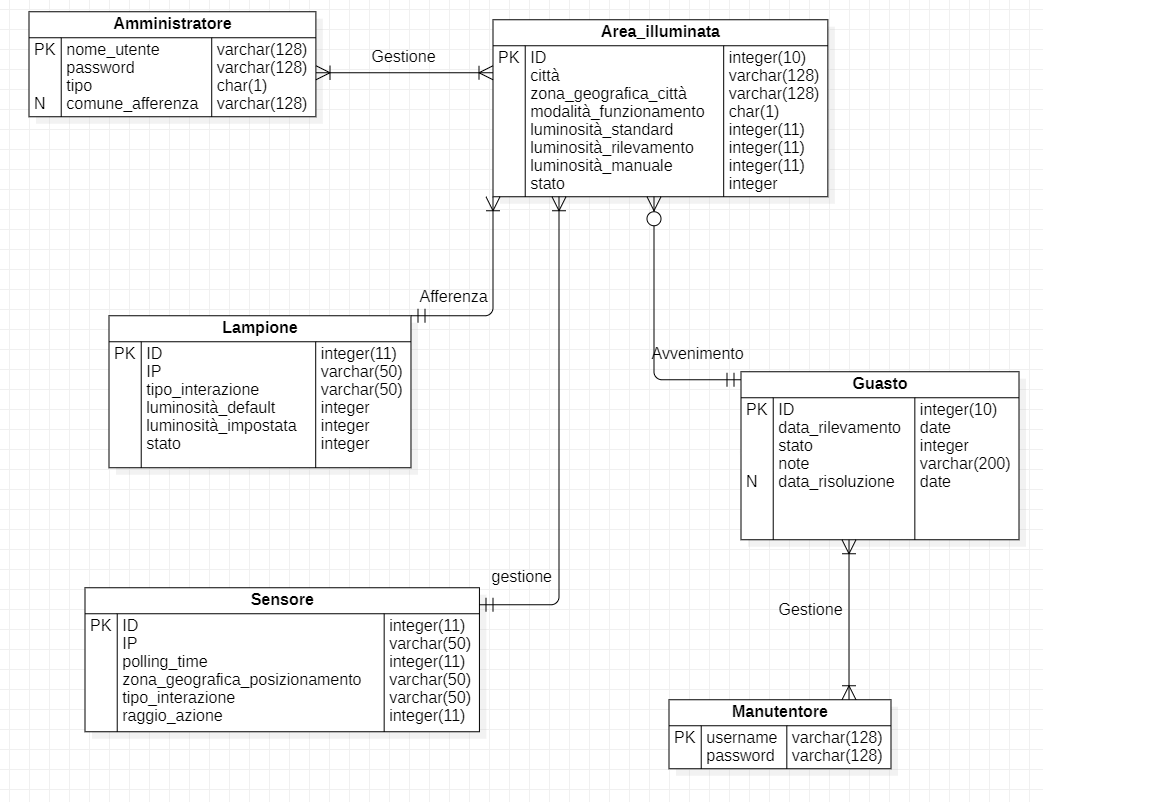
\includegraphics[width=450pt]{er ristrutturato.png}
Per poter usare efficacemente i dati salvati nel DB, il backend dell'applicazione utilzza un'apposita classe model, che tramite l'uso di Sequelize permette di creare degli oggetti di tipo lampione, area e sensore.
\subsection{Autenticazione}
Il sistema di autenticazione permette di accedere al sistema e alle Routes protette, accessibili solamente dall'amministratore.
L'autenticazione avviene tramite il check delle credenziali salvate nel database per ogni amministratore.
Dopo aver appurato che i dati inseriti siano corretti, viene generato un token di tipo JWT, a durata predeterminata. Alla scadenza del tempo prefissato tale token viene rinnovato, altrimenti se si effettua il logout, questo viene cancellato e all'accesso successivo è necessario fornire nuovamente le credenziali per l'accesso.

 	
\section{Requisiti soddisfatti}
\subsection{Tabella requisiti soddisfatti}

\begin{tabular}{ |p{1.8cm}|p{5.2cm}|p{2.5cm}| p{3.5cm}| }
	\hline
	Requisito& Descrizione &Classificazione & Stato \\
	\hline
	RF1	 & L'utente deve poter fare il login al sistema & Obbligatorio & Soddisfatto \\
	\hline				
	RF2	 & L'utente visualizza lo stato del sistema & Obbligatorio & Soddisfatto \\
	\hline				
	RF3	 & L'utente deve poter aumentare la luminosità di un'area & Obbligatorio & Soddisfatto \\
	\hline				
	RF4	 & Il sistema deve visualizzare un messaggio d'errore se non si è potuto aumentare la luminosità & Obbligatorio & Soddisfatto \\
	\hline	
	RF5 & L'utente deve poter vedere l'elenco delle aree illuminate & Obbligatorio & Soddisfatto \\
	\hline
	RF6 & L'utente deve poter vedere l'elenco delle aree & Obbligatorio & Soddisfatto \\
	\hline
	RF7	 & L'utente deve poter selezionare le aree su cui operare & Obbligatorio & Soddisfatto \\
	\hline	
	RF8	 & L'utente deve poter diminuire la luminosità di un'area & Obbligatorio & Soddisfatto \\
	\hline				
	RF10	 & L'utente deve poter accedere alla dashboard & Obbligatorio & Soddisfatto \\
	\hline										
	RF11	 & Il sistema deve visualizzare un messaggio d'errore nel caso l'operazione di diminuzione della luminosità non fosse andata a buon fine & Obbligatorio & Soddisfatto \\
	\hline				
	RF12	 & L'utente deve poter diminuire la luminosità & Obbligatorio & Soddisfatto \\
	\hline				
\end{tabular}

\begin{tabular}{ |p{1.8cm}|p{5.2cm}|p{2.5cm}| p{3.5cm}| }
	\hline
	Requisito& Descrizione &Classificazione & Stato \\
	\hline
	RF13	 & L'utente deve poter inserire una nuova area illuminata & Obbligatorio & Soddisfatto \\
	\hline
	RF14	 & L'utente deve poter rimuovere un area illuminata & Obbligatorio & Soddisfatto \\
	\hline
	RF15	 & L'utente deve poter accedere alla lista delle aree gestite & Obbligatorio & Soddisfatto \\
	\hline				
	RF16	 & L'utente deve poter modificare le informazioni di un'area illuminata	& Obbligatorio & Soddisfatto \\
	\hline				
	RF17	 & Il sistema mostra un messaggio di notifica una volta effettuata la modifica ad un area illuminata & Obbligatorio & Soddisfatto \\
	\hline				
	RF18	 & L'utente deve poter inserire un nuovo sensore in una area illuminata & Obbligatorio & Soddisfatto \\
	\hline				
	RF19	 & L'utente deve poter accedere all'area illuminata & Obbligatorio & Soddisfatto \\
	\hline 				
	RF20	 & L'utente deve poter rimuovere un sensore da un'area illuminata & Obbligatorio & Soddisfatto \\
	\hline				
	RF21	 & L'utente deve poter fare il logout dal sistema & Obbligatorio & Soddisfatto \\
	\hline										
	RF22	 & L'utente deve poter inserire un impianto nell'elenco dei guasti & Obbligatorio & Soddisfatto \\
	\hline				
	RF23	 & L'utente deve poter rimuovere un impianto dall'elenco dei guasti & Obbligatorio & Soddisfatto \\
	\hline				
	RF24	 & L'utente deve poter visualizzare i dettagli di un'area & Obbligatorio & Soddisfatto \\
	\hline				
	RF25	 & L'utente deve poter selezionare un lampione & Obbligatorio & Soddisfatto \\
	\hline				
	RF26	 & L'utente deve poter visualizzare i dettagli di un lampione & Obbligatorio & Soddisfatto \\
	\hline				
	RF27	 & L'utente deve poter inserire un nuovo lampione all'interno di un'area illuminata & Obbligatorio & Soddisfatto \\
	\hline				
	RF28	 & L'utente deve poter rimuovere un lampione all'interno di un'area illuminata & Obbligatorio & Soddisfatto \\
	\hline
\end{tabular}
	
\begin{tabular}{ |p{1.8cm}|p{5.2cm}|p{2.5cm}| p{3.5cm}| }
	\hline
	Requisito& Descrizione &Classificazione & Stato \\
	\hline	
	RF29	 & L'utente deve poter visualizzare l'elenco delle aree illuminate con dei malfunzionamenti & Obbligatorio & Soddisfatto \\
	\hline				
	RF30	 & L'amministratore deve poter aprire una nuova segnalazione di un guasto tramite un ticket & Obbligatorio & Soddisfatto \\
	\hline				
	RF31	 & L'amministratore deve poter chiudere il ticket dopo aver fatto la dovuta manutenzione & Obbligatorio & Soddisfatto \\
	\hline				
	RF32	 & Il manutentore deve poter visualizzare i dettagli aggiuntivi di un guasto forniti dal ticket & Desiderabile & Soddisfatto \\
	\hline				
	RF33	 & L'utente non amministratore riceve le credenziali da amministratore da un superamministratore & Desiderabile & Non Soddisfatto \\
	\hline				
	RF34	 & L'utente consulta il manuale Lumos Minima & Desiderabile & Soddisfatto \\
	\hline				
	RF35	 & Le nuove aree illuminate appena inserite hanno un setup standard & Desiderabile & Soddisfatto \\
	\hline				
	\end{tabular}
	Numero di requisiti obbligatori soddisfatti: 30/30 \\
	Numero di requisiti desiderabili soddisfatti: 3/4 \\
	\subsection{Qualità}
	\begin{tabular}{ |p{1.8cm}|p{5.2cm}|p{3cm}| p{2cm}| }
	\hline
	Requisito& Descrizione &Classificazione & Stato \\
	\hline
	RQ1 & La webapp deve essere sviluppata seguendo le regole descritte nel documento Norme di progetto & Obbligatorio & Soddisfatto \\
	RQ2 & Devono essere sviluppati dei test con una copertura minima dell'80\% e correlati di report & Obbligatorio & Soddisfatto\\
	RQ3 & Deve essere prodotto un documento sulle scelte implementative e progettuali & Obbligatorio & Soddisfatto \\
	RQ4 & Deve essere prodotto un documento sui problemi aperti e sulle eventuali soluzioni da esplorare & Obbligatorio & Non soddisfatto \\
	RQ5 & Fornire un’analisi rispetto al carico massimo supportato in numero di dispositivi e di quale sarebbe il servizio cloud più adatto per supportarlo analizzando prezzo, stabilità del servizio ed assistenza.  &  Facoltativo & Non soddisfatto \\
	\hline
	
	\end{tabular}
	Numero di requisiti qualitativi obbligatori soddisfatti: 3/4.\\
	Numero di requisiti qualitativi facoltativi soddisfatti: 0/1.
	\\
	\\

	Il RQ4 non è stato completato poichè non sono state rilevate particolari criticità, come confermato da Imola Informatica.
\subsection{Dati copertura test}
La piattaforma utilizzata per il testing è Jest, ed è stata utilizzata sia per i test di unità che per i test di integrazione, concordando con il committente una pecentuale minima di copertura dell'80\%.
\\Tali dati sono riproducibili eseguendo il comando "npm test" sia su frontend che su backend. I valori forniti sono le percentuali medie riscontrate, visibili nella prima riga delle percentuali del report fornito da jest.
	\subsubsection{Percentuali test}
	Dopo aver completato un'accurata fase di testing, i risultati sono i seguenti:
	\\
	\subsubsection{Test Unità}
	\begin{itemize}
		\item Statement Coverage: 87\%
		\item Branch Coverage: 81\%
		\item Function Coverage: 95\%
		\item Line Coverage: 87\%
	\end{itemize}
	\subsubsection{Test Integrazione}
	\begin{itemize}
		\item Statement Coverage: 99\%
		\item Branch Coverage: 94\%
		\item Function Coverage: 92\%
		\item Line Coverage: 99\%
	\end{itemize}

\end{document}
